\documentclass[11pt]{article}

\usepackage[margin=1in]{geometry}
\usepackage[T1]{fontenc}
\usepackage{lmodern}
\usepackage{amsmath,amssymb,amsthm}
\usepackage{booktabs}
\usepackage{enumerate}
\usepackage[font=small,labelfont=bf]{caption}
\usepackage{tikz}
\usetikzlibrary{calc, arrows.meta, decorations.pathreplacing, fit}
\usepackage[hidelinks]{hyperref}
\renewcommand{\sectionautorefname}{Section}
\renewcommand{\subsectionautorefname}{Section}

\newtheorem{theorem}{Theorem}
\newtheorem{lemma}[theorem]{Lemma}
\newtheorem{fact}[theorem]{Fact}
\newtheorem{corollary}[theorem]{Corollary}
\newtheorem{observation}[theorem]{Observation}
\theoremstyle{definition}
\newtheorem{definition}[theorem]{Definition}

% ---------------------------------------------------------------------------
% Notation
\newcommand{\Z}{\mathbb{Z}}
\newcommand{\R}{\mathbb{R}}
\newcommand{\N}{\mathbb{N}}
\newcommand{\tO}{\tilde{O}}
\renewcommand{\O}{O}
\DeclareMathOperator{\Ham}{Ham}
\DeclareMathOperator{\Match}{Match}
\DeclareMathOperator{\dom}{dom}
\DeclareMathOperator{\depth}{depth}
\newcommand{\cS}{\mathcal{S}}
\newcommand{\cV}{\mathcal{V}}
\newcommand{\cC}{\mathcal{C}}
\newcommand{\res}{\mathrm{res}}
\newcommand{\abs}[1]{\lvert #1 \rvert}
\newcommand{\inorm}[1]{\lvert #1 \rvert_\infty}
\newcommand{\x}[1]{#1.x}
\newcommand{\y}[1]{#1.y}
\newcommand{\str}[1]{\texttt{#1}}

% ---------------------------------------------------------------------------
% Drawing styles
\tikzset{
  cell/.style={draw=gray!60, minimum width=0.46cm, minimum height=0.46cm, inner sep=0pt,
    font=\ttfamily\small, anchor=center},
  mis/.style={fill=red!25},
  win/.style={draw=violet, very thick, rounded corners=1pt},
}
% A grid of characters; rows are given from top to bottom.
% \chargrid{x offset}{y offset}{row_top,...,row_bottom}
\newcommand{\chargrid}[3]{%
  \foreach \row [count=\r] in {#3} {
    \foreach \ch [count=\c] in \row {
      \node[cell] at ({#1+(\c-1)*0.46}, {#2-(\r-1)*0.46}) {\ch};
    }
  }%
}

\title{Two-Dimensional Pattern Matching with $k$ Mismatches}
\author{}
\date{}

\begin{document}
\maketitle

\section{Introduction}

Suppose we are given an image, a two-dimensional array of characters, and a smaller template, and we want to find all places where the template appears in the image.
If the template must appear exactly, this is two-dimensional exact pattern matching, which can be solved in linear time.
Real data is noisy, so we rather want to find all places where the template appears \emph{up to at most $k$ mismatched cells}.

Formally, the \emph{text} $T$ is an $n \times n$ array and the \emph{pattern} $P$ is an $m \times m$ array, with $m \le n$.
For every \emph{position} $q$, that is, every placement of the pattern inside the text, we want to know the number of cells in which the pattern differs from the text below it, or that this number exceeds~$k$.
\autoref{fig:problem} shows an example, which we will use as our running example.

\begin{figure}[t]
  \centering
  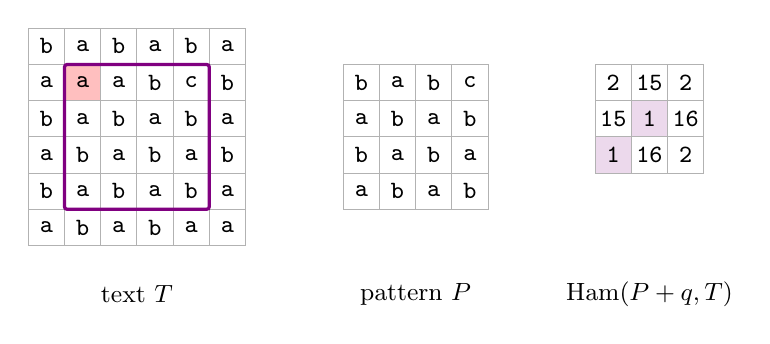
\begin{tikzpicture}
    % text, rows from top (y=5) to bottom (y=0)
    \chargrid{0}{0}{{b,a,b,a,b,a},{a,a,a,b,c,b},{b,a,b,a,b,a},{a,b,a,b,a,b},{b,a,b,a,b,a},{a,b,a,b,a,a}}
    \node[cell, mis] at (1*0.46, -1*0.46) {a};
    \node[win, fit={(0.46-0.23, -0.46+0.23) (4*0.46+0.23, -4*0.46-0.23)}, inner sep=0pt] {};
    \node[font=\small] at (1.15, -3.15) {text $T$};
    % pattern
    \chargrid{4.0}{-0.46}{{b,a,b,c},{a,b,a,b},{b,a,b,a},{a,b,a,b}}
    \node[font=\small] at (4.0+0.69, -3.15) {pattern $P$};
    % table of distances, rows q.y = 2,1,0 from top
    \begin{scope}[xshift=7.2cm, yshift=-0.46cm]
      \chargrid{0}{0}{{2,15,2},{15,1,16},{1,16,2}}
      \node[cell, fill=violet!15] at (0, -2*0.46) {1};
      \node[cell, fill=violet!15] at (0.46, -0.46) {1};
    \end{scope}
    \node[font=\small, align=center] at (7.2+0.46, -3.15) {$\Ham(P+q,T)$};
  \end{tikzpicture}
  \caption{A text $T$ with $n = 6$ and a pattern $P$ with $m = 4$, drawn with the $y$-axis pointing up, so that the cell $(0,0)$ is at the bottom left.
    The window (violet) shows the pattern at position $q = (1,1)$; it has one mismatch (red), since $P(0,3) = \str{b}$ lies on $T(1,4) = \str{a}$.
    Right: the Hamming distances for all nine positions $q \in [3]^2$, again with $q = (0,0)$ at the bottom left.
    For $k = 1$, the positions $(0,0)$ and $(1,1)$ (shaded) are reported.
    Both $P$ and $T$ are close to the checkerboard pattern; this periodicity will be central to the algorithm.}
  \label{fig:problem}
\end{figure}

The classical algorithm of Amir and Landau solves this problem in $\O(kn^2)$ time.
In these notes, we show the following.

\begin{theorem}\label{thm:main}
  The problem can be solved in $\tO(n^2 + kn^2/m)$ time.
  In particular, it can be solved in $\tO(n^2)$ time if $k = \O(m)$.
\end{theorem}

This bound is the natural two-dimensional analogue of the one-dimensional bound $\tO(N + kN/\sqrt{M})$ of Gawrychowski and Uzna\'nski for a text of length $N = n^2$ and a pattern of length $M = m^2$.
In \autoref{sec:lower}, we show that it is optimal for combinatorial algorithms, assuming the combinatorial BMM hypothesis.

\paragraph{The idea in a nutshell.}
It suffices to consider $n \le \frac32 m$.
A standard filter finds a set $Q$ of candidate positions, each with at most $2k$ mismatches.
If $Q$ is small, we check the candidates one by one.
Otherwise, two candidates are close to each other, and their difference is an \emph{approximate period} of the pattern: shifting $P$ by it creates few mismatches.
We find two such periods $\phi$ and $\psi$, which span a lattice with $\O(k)$ cosets.
Along these periods, the pattern changes its character only $\O(k)$ times, so it splits into $\O(k)$ monochromatic pieces of a simple shape.

The text is the difficult part: only the region $A$ covered by the candidates matters, but $A$ is \emph{not} approximately periodic as a whole.
However, a small piece of $A$ that is far from the boundary of $A$, relative to its size, lies inside a single candidate occurrence and therefore inherits the periodicity of the pattern.
So we cut $A$ into cells whose size is proportional to their distance to the boundary.
At distance about $D$, there are $\O(m/D)$ cells, each splits into $\O(k)$ monochromatic pieces, and the matches between text pieces and pattern pieces can be counted in two ways, for each character separately:
by enumerating all pairs of pieces, or by FFT.
The FFT is cheap close to the boundary: a text cell at distance $D$ from the boundary of $A$ can only lie below a strip of width $\O(D)$ along the boundary of the pattern, so the FFT takes $\tO(mD)$ time.

\paragraph{Where the bound comes from.}
At every distance $D$, the number of text pieces times the FFT cost is $\O(mk/D) \cdot \tO(mD) = \tO(m^2 k)$, independently of $D$.
Choosing the cheaper method for each character, the Cauchy--Schwarz inequality bounds the total cost by $\tO(\sqrt{m^2 k \cdot k}) = \tO(mk)$ per distance.
With $\O(\log m)$ distances and $\O(n^2/m^2)$ texts of size $\frac32 m$, this gives \autoref{thm:main}.

\autoref{tab:results} compares the bounds.

\begin{table}[ht]
  \centering
  \renewcommand{\arraystretch}{1.3}
  \begin{tabular}{@{}lll@{}}
    \toprule
    & time & quasi-linear for \\
    \midrule
    Amir and Landau & $\O(kn^2)$ & $k = \O(\log n)$ \\
    previous version of this work & $\tO(n^2 + k^{5/4} n^2/m)$ & $k = \O(m^{4/5})$ \\
    these notes & $\tO(n^2 + kn^2/m)$ & $k = \O(m)$ \\
    lower bound (combinatorial) & $(kn^2/m)^{1-o(1)}$ & --- \\
    \bottomrule
  \end{tabular}
  \caption{Bounds for two-dimensional pattern matching with $k$ mismatches, for an $n \times n$ text and an $m \times m$ pattern.
    The lower bound holds for $m < k \le m^2$ and assumes the combinatorial BMM hypothesis.}
  \label{tab:results}
\end{table}

\section{Preliminaries}

We work in the word RAM model; the alphabet $\Sigma$ consists of integers polynomial in $n$, and $\tO$ hides factors polylogarithmic in $n$.
For $m \in \Z^+$, let $[m] = \{0, \dots, m-1\}$.

\paragraph{Geometry.}
A point $u \in \Z^2$ has coordinates $u = (\x u, \y u)$, and we draw the $y$-axis pointing up.
For $u, v \in \R^2$, let $\det(u,v) = \x{u}\,\y{v} - \y{u}\,\x{v}$; it is positive if $v$ lies counterclockwise from $u$.
We write $\abs{u}$ for the Euclidean norm and $\inorm{u}$ for the maximum norm.

\paragraph{Strings.}
It is convenient to allow arbitrary shapes.
A \emph{string} is a partial function $S \colon \Z^2 \rightharpoonup \Sigma$ with finite domain $\dom(S)$.
For $X \subseteq \Z^2$, $S|_X$ is the restriction of $S$ to $\dom(S) \cap X$.
For $\delta \in \Z^2$, $S + \delta$ is the string with $\dom(S+\delta) = \dom(S) + \delta$ and $(S+\delta)(u) = S(u - \delta)$; that is, we move $S$ by $\delta$.
For strings $S, R$ and $c \in \Sigma$, we count mismatches and matches with character $c$ where both strings are defined:
\begin{align*}
\Ham(S,R) &= \abs{\{u \in \dom(S) \cap \dom(R) : S(u) \neq R(u)\}},\\
\Match_c(S,R) &= \abs{\{u \in \dom(S) \cap \dom(R) : S(u) = R(u) = c\}}.
\end{align*}
A string $S$ is \emph{monochromatic} with character $c(S)$ if $S(u) = c(S)$ for all $u \in \dom(S)$.

\paragraph{The problem.}
We are given a pattern $P$ with $\dom(P) = [m]^2$, a text $T$ with $\dom(T) = [n]^2$, $m \le n$, and $k \in \Z^+$.
For every position $q \in [n-m+1]^2$, we compute $\min\{k+1, \Ham(P+q, T)\}$.

\subsection{Tools}

\begin{fact}[FFT]\label{fact:fft}
Let $S, R$ be strings with domains contained in axis-parallel rectangles of sizes $w_S \times h_S$ and $w_R \times h_R$, respectively, and let $c \in \Sigma$. The values $\Match_c(S, R + q)$ for all $q \in \Z^2$ (all but $N = (w_S + w_R)(h_S + h_R)$ of which are zero) can be computed in $\O(N \log N)$ time.
\end{fact}

\begin{fact}[Karloff's algorithm]\label{fact:karloff}
In $\tO(n^2)$ time, one can compute values $h(q)$ with $\Ham(P+q,T) \le h(q) \le 2\Ham(P+q,T)$ for all $q \in [n-m+1]^2$.
\end{fact}
(Karloff's algorithm reduces the problem to $\O(\log^2 n)$ instances over the binary alphabet, each of which is solved with Fact~\ref{fact:fft}; nothing in it is specific to one dimension.)

\begin{fact}[Offline range counting]\label{fact:range}
Given $N$ weighted axis-parallel boxes in $\R^4$ and $M$ points in $\R^4$, the total weight of the boxes containing each point can be computed in $\O((N + M)\log^4(N+M))$ time.
\end{fact}

\begin{lemma}[Kangaroo jumps]\label{lem:kangaroo}
Given $Q' \subseteq [n-m+1]^2$, one can compute $\min\{k+1, \Ham(P+q, T)\}$ for all $q \in Q'$ in $\O(n^2 + \abs{Q'} k)$ time.
\end{lemma}
\begin{proof}
For $x \in [m]$, let $p_x$ be column $x$ of $P$, a one-dimensional string of length $m$. For $x \in [n]$ and $y \in [n-m+1]$, let $t_{x,y}$ be the length-$m$ substring of column $x$ of $T$ starting in row $y$. Then $\Ham(P+q, T) = \sum_{x \in [m]} \Ham(p_x, t_{\x{q}+x, \y{q}})$, where $\Ham$ of one-dimensional strings is defined in the natural way. Build the suffix tree of the concatenation of all columns of $P$ and $T$ (separated by unique delimiters), augmented for constant-time longest common extension (LCE) queries. This takes $\O(n^2)$ time and allows assigning integer identifiers $\iota(\cdot)$ to the strings $p_x$ and $t_{x,y}$ such that two of them are equal if and only if their identifiers are equal. For every $y$, build the LCE structure also for the one-dimensional strings $\iota(t_{0,y}) \cdots \iota(t_{n-1,y})$ and $\iota(p_0) \cdots \iota(p_{m-1})$ (total length $\O(n^2)$). Now fix $q \in Q'$. With LCE queries on the identifier strings, we enumerate the columns $x$ with $\iota(p_x) \neq \iota(t_{\x{q}+x,\y{q}})$ in $\O(1)$ time each, and for every such $x$, we enumerate the mismatches between $p_x$ and $t_{\x{q}+x,\y{q}}$ in $\O(1)$ time each. We stop after $k+1$ mismatches. Every enumerated column contains a mismatch, so this takes $\O(k + 1)$ time per $q$.
\end{proof}

\section{Filtering and two periods}

\paragraph{Assumptions.} We may assume $n \le 3m/2$: otherwise, we cover $[n-m+1]^2$ with $\O(n^2/m^2)$ translates of $[n'-m+1]^2$, where $n' = \lfloor 3m/2 \rfloor$, and solve the instance with text $T|_{[n']^2 + \delta}$ for every such translate $[n'-m+1]^2 + \delta$. We also assume that $m$ is larger than a suitable constant (otherwise, the naive algorithm takes $\O(n^2)$ time). It thus suffices to give an $\tO(m^2 + mk)$-time algorithm. Let $\ell = n - m \le m/2$, so that the set of positions is $[\ell+1]^2$.

\paragraph{Filtering.} We compute the values $h(q)$ of Fact~\ref{fact:karloff} and let $Q = \{q : h(q) \le 2k\}$. Then every $q$ with $\Ham(P+q,T) \le k$ is in $Q$, and $\Ham(P+q,T) \le 2k$ for every $q \in Q$. For every $q \notin Q$, the answer is $k+1$. If $\abs{Q} \le 32m + m^2/k$, we finish with Lemma~\ref{lem:kangaroo} in $\O(m^2 + mk)$ time. From now on, we assume $\abs{Q} > 32m + m^2/k$.

\begin{lemma}\label{lem:period}
For all $u, v \in Q$, we have $\Ham(P + (u - v), P) \le 4k$.
\end{lemma}
\begin{proof}
$\Ham(P+u-v, P) = \Ham(P+u, P+v) \le \Ham(P+u, T) + \Ham(T, P+v) \le 4k$, since every $w \in \dom(P+u) \cap \dom(P+v) \subseteq \dom(T)$ with $(P+u)(w) \ne (P+v)(w)$ is a mismatch between $T$ and $P+u$ or between $T$ and $P+v$.
\end{proof}

\begin{lemma}[Two periods]\label{lem:two_periods}
Let $\ell \ge 1$ and $U \subseteq [\ell+1]^2$ with $\abs{U} \ge 32\ell$. In $\O(\abs{U}\log\abs{U})$ time, one can find $\phi, \psi \in U - U$ with $\psi \in (0, \infty) \times [0, \infty)$, $\phi \in [0, \infty) \times (-\infty, 0)$, $\det(\phi,\psi) \ge \frac12\abs{\phi}\abs{\psi}$, and $\abs{\phi}\abs{\psi} < 30\ell^2/\abs{U}$.
\end{lemma}
\begin{proof}
Note that $U - U = -(U-U)$. Let $r$ be the minimum distance between two distinct points of $U$, and let $w \in U - U$ with $\abs{w} = r$ (a closest pair can be found in $\O(\abs{U}\log\abs{U})$ time).
If $r > \ell/\sqrt 2$, then each of the four closed quarters of $[0,\ell]^2$ (of diameter $\ell/\sqrt2$) contains at most one point of $U$, contradicting $\abs{U} > 4$. Hence $r \le \ell$. The open disks of radius $r/2$ centred at the points of $U$ are disjoint and contained in $[-r/2, \ell + r/2]^2$, so $\abs{U} \pi r^2/4 \le 4\ell^2$ and $r^2 < 6\ell^2/\abs{U}$.

Let $\theta \in [0^\circ, 180^\circ)$ be the angle of the line through $w$. If $\theta < 90^\circ$, let $e = (1,1)$ and $e' = (-1,1)$; otherwise, let $e = (1,-1)$ and $e' = (1,1)$. Let $a = r/4$ and $b = 28\ell^2/(r\abs{U})$; note that $b \le \ell$ because $r \ge 1$ and $\abs{U} \ge 28\ell$. We put every $u \in U$ into the bucket $(\lfloor (u \cdot e)/a \rfloor, \lfloor (u \cdot e')/b\rfloor)$. As $u \cdot e$ and $u \cdot e'$ range over intervals of length $2\ell$, there are at most $(2\ell/a + 1)(2\ell/b+1) \le (9\ell/r)(3\ell/b) = \frac{27}{28}\abs{U}$ non-empty buckets. Hence, some bucket contains two distinct points, and their difference $w' \in U - U$ satisfies $\abs{w' \cdot e} < a$, $\abs{w'\cdot e'} < b$, and $\abs{w'} \ge r$. Thus $\abs{w'}^2 = ((w' \cdot e)^2 + (w'\cdot e')^2)/2 < (a+b)^2$, and
\[\abs{w}\abs{w'} < r(a + b) = r^2/4 + 28\ell^2/\abs{U} < 30\ell^2/\abs{U}.\]
Moreover, the angle $\beta$ between $w'$ and the line orthogonal to $e$ satisfies $\sin\beta = \abs{w'\cdot e}/(\sqrt2\abs{w'}) < a/(\sqrt 2 r) < \sin 11^\circ$.

If $\theta < 90^\circ$, the line through $w'$ has angle in $(124^\circ, 146^\circ)$. We let $\psi = \pm w$ with angle in $[0^\circ, 90^\circ)$ and $\phi = \pm w'$ with angle in $(304^\circ, 326^\circ)$. If $\theta \ge 90^\circ$, the line through $w'$ has angle in $(34^\circ, 56^\circ)$, and we let $\psi = \pm w'$ with angle in $(34^\circ,56^\circ)$ and $\phi = \pm w$ with angle in $[270^\circ, 360^\circ)$. In both cases, $\psi$ and $\phi$ lie in the claimed quadrants, and the counterclockwise angle from $\phi$ to $\psi$ is in $(34^\circ, 146^\circ)$, hence $\det(\phi,\psi) = \abs{\phi}\abs{\psi}\sin(\angle(\phi,\psi)) \ge \frac12\abs{\phi}\abs{\psi}$.
\end{proof}

We apply Lemma~\ref{lem:two_periods} to $U = Q$ (note $\abs{Q} > 32m \ge 64\ell$) and fix $\phi, \psi$ for the rest of the paper. Let $\Delta = \det(\phi,\psi) \in \Z$. We have
\[ 1 \le \Delta \le \abs{\phi}\abs{\psi} \le 2\Delta, \qquad \Delta < 30\ell^2/\abs{Q} < 30 \ell^2 k / m^2 < 8k,\qquad \inorm{\phi}, \inorm{\psi} \le \ell, \]
and, by Lemma~\ref{lem:period}, $\Ham(P + \phi, P) \le 4k$ and $\Ham(P + \psi, P) \le 4k$. Recall that $\x\phi \ge 0 > \y\phi$ and $\x\psi > 0$, $\y\psi \ge 0$.

\section{Lattice blocks}

Let $L = \{i\phi + j\psi : i, j \in \Z\}$. We write $u \equiv v$ if $u - v \in L$; the congruence classes are the cosets $\gamma + L$. Let
\[\kappa(u) = (\det(u, \psi), \det(\phi, u)) \in \Z^2 \quad\text{for } u \in \Z^2.\]
Since $u = (\kappa_1(u)\phi + \kappa_2(u)\psi)/\Delta$, we have $u \equiv v$ if and only if $\kappa(u) \equiv \kappa(v) \pmod \Delta$ (componentwise), and $\kappa(\gamma + i\phi + j\psi) = \kappa(\gamma) + \Delta\cdot(i,j)$. In particular, congruence classes can be computed in constant time per point.

\begin{definition}
A \emph{block} is a set $\gamma + I\phi + J\psi := \{\gamma + i\phi + j\psi : i \in I, j \in J\}$, where $\gamma \in \Z^2$ and $I, J \subseteq \Z$ are (possibly unbounded) intervals. A \emph{tile} is a set $\{u \in \Z^2 : \kappa(u) \in X\}$, where $X \subseteq \R^2$ is a (possibly unbounded) axis-parallel box. A rectangle $R = ([x_0, x_1] \times [y_0, y_1]) \cap \Z^2$ is \emph{wide} if $x_1 - x_0 + 1 \ge \abs{\x\phi} + \abs{\x\psi}$ and $y_1 - y_0 + 1 \ge \abs{\y\phi} + \abs{\y\psi}$; we also call $R = \Z^2$ wide. A \emph{truncated block} is a set $R \cap B$, where $R$ is a wide rectangle and $B$ is a block.
\end{definition}

The intersection of a tile with a congruence class is a block. For a set $X \subseteq \Z^2$, the \emph{lattice graph} of $X$ has vertex set $X$ and edges $\{u, u+\phi\}$ and $\{u, u+\psi\}$ for all $u$ such that both endpoints are in $X$.

\begin{lemma}\label{lem:connected}
The lattice graph of every truncated block is connected.
\end{lemma}
\begin{proof}
Let $X = R \cap B$ with $R = [x_0, x_1] \times [y_0, y_1]$ wide (the case $R = \Z^2$ is trivial) and $B = \gamma + I\phi + J\psi$. For $u = \gamma + i\phi + j\psi$, write $c(u) = (i,j)$. It suffices to show that for distinct $u, v \in X$, one of them has a neighbour $w \in X$ with $\abs{c(w) - c(z)}_1 < \abs{c(u) - c(v)}_1$, where $z$ is the other of the two points. All candidates $w$ below satisfy that $c(w)$ lies in the bounding box of $c(u)$ and $c(v)$, so $w \in B$, and only $w \in R$ needs to be checked. By symmetry, assume $v = u + \alpha\phi + \beta\psi$ with $\alpha \ge 0$.

\emph{Case $\beta \ge 0$.} The $x$-coordinate does not decrease along $\phi$- and $\psi$-steps, so every $w \in \{u+\phi, u+\psi\}$ satisfies $\x u \le \x w \le \x v$. If $\beta = 0$, then $w = u + \phi$ satisfies $\y v \le \y w \le \y u$, so $w \in R$. If $\alpha = 0$, then $w = u + \psi$ satisfies $\y u \le \y w \le \y v$. If $\alpha,\beta > 0$ and $u + \phi \notin R$, then $\y u + \y\phi < y_0$, and hence $y_0 \le \y u \le \y u + \y\psi \le y_0 - 1 + \abs{\y\phi} + \abs{\y\psi} \le y_1$, so $w = u + \psi \in R$.

\emph{Case $\beta < 0$.} If $\alpha = 0$, then $w = u - \psi$ lies between $u$ and $v$ in both coordinates. Otherwise, both $u + \phi$ and $u - \psi$ have their $y$-coordinate in $[\y v, \y u]$, as $\y\phi < 0$ and $\y\psi \ge 0$. Moreover, $\x{(u+\phi)} \ge x_0$ and $\x{(u-\psi)} \le x_1$. If neither of them is in $R$, then $\x u + \x\phi > x_1$ and $\x u - \x\psi < x_0$, so $x_1 - x_0 + 2 \le \x\phi + \x\psi$, contradicting wideness.
\end{proof}

\begin{lemma}[Decomposition]\label{lem:decomposition}
Let $R$ be a wide rectangle, let $Y$ be a tile, and let $S$ be a string with $\dom(S) = R \cap Y$. Let $h = \Ham(S + \phi, S) + \Ham(S+\psi, S)$. In $\O(\abs{\dom(S)}\log \abs{\dom(S)})$ time, $S$ can be partitioned into at most $\Delta + h$ monochromatic strings whose domains are truncated blocks of the form $R \cap B$. If $R = \Z^2$, these domains are blocks.
\end{lemma}
\begin{proof}
We group $\dom(S)$ by congruence class. For every class $\gamma + L$ meeting $\dom(S)$, we have $\dom(S) \cap (\gamma + L) = R \cap (\gamma + I\phi + J\psi)$ for intervals $I, J$. Call an edge $\{u, u + \delta\}$ of the lattice graph of $\dom(S)$, $\delta \in \{\phi,\psi\}$, a \emph{$\delta$-mismatch} if $S(u) \neq S(u+\delta)$; there are $h$ mismatches in total. First, for every class, we cut $I$ between $i$ and $i+1$ for every $\phi$-mismatch $\{u, u+\phi\}$ with $c(u) = (i,j)$. This yields at most $\Delta + \Ham(S+\phi,S)$ sets $R \cap (\gamma + I'\phi + J\psi)$, none of which contains a $\phi$-mismatch. Then, we cut the $J$-interval of each of these sets at the $\psi$-mismatches it contains, which yields at most $\Delta + h$ truncated blocks $R \cap (\gamma + I'\phi + J'\psi)$ that contain no mismatch. By Lemma~\ref{lem:connected}, each of them is connected in its lattice graph, so $S$ restricted to it is monochromatic. Sorting dominates the running time.
\end{proof}

Since $\abs{\x\phi} + \abs{\x\psi} \le 2\ell \le m$ (and similarly for the $y$-coordinates), the square $[m]^2$ is wide. We apply Lemma~\ref{lem:decomposition} to $P$ with $R = [m]^2$ and $Y = \Z^2$, with $h \le 8k$. This yields a partition of $P$ into a set $\cV$ of $\abs{\cV} \le \Delta + 8k < 16k$ monochromatic strings, whose domains are truncated blocks $[m]^2 \cap B$. For $c \in \Sigma$, let $\cV_c = \{V \in \cV : c(V) = c\}$.

\section{The active text}

Let $A = \bigcup_{q \in Q}([m]^2 + q) \subseteq [n]^2$. For $q \in Q$, we have $\dom(P+q) \subseteq A$, and hence
\begin{equation}\label{eq:ham_match}
\Ham(P+q, T) = m^2 - \textstyle\sum_{c \in \Sigma} \Match_c(P + q, T|_A).
\end{equation}
For $u \in \Z^2$, let $\depth(u) = \min\{\inorm{u - v} : v \in \Z^2 \setminus A\}$; in particular, $\depth(u) = 0$ for $u \notin A$, and $\abs{\depth(u) - \depth(v)} \le \inorm{u - v}$. The depths of all $u \in [n]^2$ can be computed in $\O(n^2)$ time by a breadth-first search from $[-1,n]^2 \setminus A$ in the king's graph.

\begin{lemma}[Coverable sets]\label{lem:coverable}
Let $X \subseteq \Z^2$ with $\inorm{u-v} \le r < m/2$ for all $u, v \in X$, and $\depth(u) > r$ for all $u \in X$. Then $X \subseteq [m]^2 + q$ for some $q \in Q$. Consequently, $\Ham(T|_X + \delta, T|_X) \le 8k$ for $\delta \in \{\phi,\psi\}$.
\end{lemma}
\begin{proof}
Let $[x_0, x_1]$ and $[y_0, y_1]$ be the ranges of the $x$- and $y$-coordinates of $X$. As $x_1 - x_0 \le r < m - \ell$, we have $x_0 \ge \ell$ or $x_1 \le m - 1$, and similarly for $y$. Assume $x_0, y_0 \ge \ell$; the other three cases are symmetric (using the corresponding corner of the bounding box). The corner $(x_1, y_1)$ is within distance $r$ of a point of $X$, and hence it is in $A$, that is, in $[m]^2 + q$ for some $q \in Q \subseteq [\ell+1]^2$. For every $u \in X$, we have $\x q \le \ell \le x_0 \le \x u \le x_1 \le \x q + m - 1$, and similarly for $y$. Thus $X \subseteq [m]^2 + q$.

For the second claim, if $u - \delta, u \in X$ and $T(u-\delta) \ne T(u)$, then $T(u - \delta) \neq P(u - \delta - q)$, or $P(u-\delta-q) \neq P(u-q)$, or $P(u-q) \neq T(u)$. Thus $\Ham(T|_X + \delta, T|_X) \le \Ham(P+q,T) + \Ham(P+\delta,P) + \Ham(P+q,T) \le 8k$.
\end{proof}

Let $z = \lceil n/2 \rceil$. The \emph{quarters} are $K_1 = [z,\infty)^2$, $K_2 = (-\infty, z) \times [z, \infty)$, $K_3 = (-\infty, z)^2$, and $K_4 = [z, \infty) \times (-\infty, z)$ (intersected with $\Z^2$). We state the following for $K_1$; the statements for the other quarters are symmetric (reflect the coordinates as appropriate; for $K_3$, for instance, the condition $\ell \le \x w \le \x v$ becomes $\x v \le \x w \le m - 1$).

\begin{lemma}\label{lem:monotone}
\begin{enumerate}[(a)]
\item If $v \in A$ and $\ell \le \x w \le \x v$ and $\ell \le \y w \le \y v$, then $w \in A$.
\item If $d \le m/8$, $u \in A \cap K_1$, and $\depth(u) \le d$, then $u + (d,d) \notin A$.
\end{enumerate}
\end{lemma}
\begin{proof}
(a) If $v \in [m]^2 + q$ with $q \in [\ell+1]^2$, then $\x q \le \ell \le \x w \le \x v \le \x q + m - 1$ and likewise for $y$, so $w \in [m]^2 + q$. (b) Every $w \in u + [-d,d]^2$ has coordinates at least $z - d \ge n/2 - m/8 \ge n - m = \ell$ (using $n \le 3m/2$). If $u + (d,d) \in A$, then (a) gives $u + [-d,d]^2 \subseteq A$, that is, $\depth(u) > d$.
\end{proof}

\begin{lemma}[Shallow points]\label{lem:shallow}
For every $d \ge 1$, $\abs{\{u \in A : \depth(u) \le d\}} = \O(md)$.
\end{lemma}
\begin{proof}
If $d > m/8$, the bound follows from $\abs{A} \le n^2 = \O(m^2)$. Otherwise, consider $K_1$ (the other quarters are symmetric) and a diagonal line $\{u_0 + t(1,1) : t \in \Z\}$. By Lemma~\ref{lem:monotone}(a), the points of $A \cap K_1$ on this line form a prefix (with respect to $t$) of the points of $K_1$ on this line. By Lemma~\ref{lem:monotone}(b), at most $d$ points $u$ of this prefix satisfy $\depth(u) \le d$. At most $2n$ diagonal lines meet $[n]^2$.
\end{proof}

\section{Multiscale decomposition of the active text}

Let $D_j = 16 \cdot 2^j$ for $j \in \{0, \dots, J\}$, where $J$ is the largest integer with $D_J \le m/16$. For $j \in \{0, \dots, J\}$ and $a, b \in \Z$, the \emph{level-$j$ cell} with index $(a,b)$ is the tile
\[ \{u \in \Z^2 : \kappa_1(u) \in [a, a+1) \cdot D_j\Delta/\abs{\phi},\ \kappa_2(u) \in [b, b+1)\cdot D_j\Delta/\abs{\psi}\}. \]
Geometrically, this is the set of integer points in a half-open rhombus with sides $D_j\phi/\abs{\phi}$ and $D_j\psi/\abs{\psi}$. We use the following properties.
\begin{enumerate}[(C1)]
\item The level-$j$ cells partition $\Z^2$, and each level-$(j+1)$ cell is the union of four level-$j$ cells (its \emph{children}).
\item Any two points of a level-$j$ cell have distance at most $2D_j$.
\item Each level-$j$ cell contains at least $D_j^2/16$ points: since the angle between $\phi$ and $\psi$ has sine at least $1/2$, the rhombus contains an open disk of radius $D_j/4$, hence an open axis-parallel square of side $D_j/(2\sqrt2) \ge D_j/4 + 1$.
\end{enumerate}

A level-$j$ cell $C$ is \emph{good} if $\depth(u) > 2D_j$ for all $u \in C$. By (C2) and Lemma~\ref{lem:coverable} (with $r = 2D_j \le m/8$), every good cell is contained in $[m]^2 + q$ for some $q \in Q$. The children of a good cell are good. A good level-$j$ cell is \emph{selected} if $j = J$ or its parent is not good. The selected cells are pairwise disjoint. For $j \in \{0, \dots, J\}$, let $A_j$ be the union of the selected level-$j$ cells, and let $A_\res = A \setminus \bigcup_j A_j$. We call $\res, 0, \dots, J$ the \emph{levels}, and we define the \emph{depth bounds} $d_\res = 4D_0$, $d_j = 8D_j$ for $j < J$, and $d_J = n$.

\begin{lemma}\label{lem:levels}
For every level $\iota$, every $u \in A_\iota$ satisfies $\depth(u) \le d_\iota$. Moreover, $\abs{A_\res} = \O(m)$, and there are $\O(m/D_j)$ selected level-$j$ cells for every $j \in \{0, \dots, J\}$.
\end{lemma}
\begin{proof}
Let $j < J$, and let $u$ be in a selected level-$j$ cell with parent $C'$. As $C'$ is not good, some $u' \in C'$ has $\depth(u') \le 2D_{j+1}$, and $\inorm{u - u'} \le 2D_{j+1}$ by (C2), so $\depth(u) \le 4D_{j+1} = 8D_j$. The selected level-$j$ cells are disjoint, contain at least $D_j^2/16$ points each by (C3), and these points have depth at most $8D_j$; by Lemma~\ref{lem:shallow}, there are $\O(mD_j)/(D_j^2/16) = \O(m/D_j)$ such cells. For $j = J$, the bound $d_J = n$ is trivial, and there are at most $16n^2/D_J^2 = \O(1)$ selected level-$J$ cells.

Now let $u \in A_\res$. If the level-$0$ cell of $u$ were good, then its highest good ancestor (of level at most $J$) would be selected and would contain $u$. Hence some $u'$ in the level-$0$ cell of $u$ has $\depth(u') \le 2D_0$, and thus $\depth(u) \le 4D_0$. By Lemma~\ref{lem:shallow}, $\abs{A_\res} = \O(m)$.
\end{proof}

\paragraph{Text blocks.} For every selected cell $C$, the string $T|_C$ has domain $C$, a tile, and by Lemma~\ref{lem:coverable}, $\Ham(T|_C + \delta, T|_C) \le 8k$ for $\delta \in \{\phi,\psi\}$. By Lemma~\ref{lem:decomposition} (with $R = \Z^2$), $T|_C$ can be partitioned into at most $\Delta + 16k < 24k$ monochromatic strings whose domains are blocks. For $j \in \{0,\dots,J\}$, let $\cS_j$ be the set of all such strings obtained from the selected level-$j$ cells, and let $\cS_\res = \{T|_{\{u\}} : u \in A_\res\}$ (a singleton is a block). For every level $\iota$ and $c \in \Sigma$, let $\cS_{\iota,c} = \{S \in \cS_\iota : c(S) = c\}$. By Lemma~\ref{lem:levels}, for every level $\iota$,
\begin{equation}\label{eq:pieces}
\abs{\cS_\iota} \cdot d_\iota = \O(mk).
\end{equation}
All of this takes $\tO(m^2 + mk)$ time: the depths, cells, and selected cells are computed in $\tO(n^2)$ time, every point of $A$ is processed by Lemma~\ref{lem:decomposition} at most once, and $\sum_\iota \abs{\cS_\iota} = \tO(mk)$.

\section{Counting matches}

For a level $\iota$, a character $c$, and $q \in [\ell+1]^2$, let
\[ M_{\iota,c}(q) = \Match_c(P + q, T|_{A_\iota}) = \sum_{S \in \cS_{\iota,c}}\ \sum_{V \in \cV_c} \abs{\dom(S) \cap \dom(V+q)}. \]
Since the sets $A_\iota$ partition $A$, (\ref{eq:ham_match}) gives $\Ham(P + q, T) = m^2 - \sum_\iota \sum_c M_{\iota,c}(q)$ for every $q \in Q$. We provide two ways of computing the values $M_{\iota,c}(q)$.

\begin{lemma}[Pairing]\label{lem:pairing}
Given a set $\Pi$ of pairs $(\iota, c)$, the values $\sum_{(\iota,c) \in \Pi} M_{\iota,c}(q)$ for all $q \in [\ell+1]^2$ can be computed in $\tO(m^2 + N)$ time, where $N = \sum_{(\iota,c) \in \Pi} \abs{\cS_{\iota,c}}\cdot\abs{\cV_c}$.
\end{lemma}
\begin{proof}
For $p \in \Z^2$, let $\cC(p) = \{p + i\phi + j\psi : i,j \ge 0\}$ be the \emph{cone} at $p$. Write the domain of every text block $S$ as $\gamma + [i_0, i_1)\phi + [j_0, j_1)\psi$ and let $w_{ab}(S) = \gamma + i_a\phi + j_b\psi$ for $a,b \in \{0,1\}$. Then, by inclusion--exclusion, $\mathbf{1}_{\dom(S)} = \sum_{a,b \in \{0,1\}} (-1)^{a+b}\,\mathbf 1_{\cC(w_{ab}(S))}$. Moreover, for every $V$, $w$, and $q$, the map $u \mapsto u - q - w$ gives $\abs{\cC(w) \cap \dom(V+q)} = \abs{\cC(-q) \cap (\dom(V) - w)}$. Hence, defining $F \colon \Z^2 \to \Z$ by
\[ F = \sum_{(\iota,c) \in \Pi}\ \sum_{S \in \cS_{\iota,c}}\ \sum_{V \in \cV_c}\ \sum_{a,b \in \{0,1\}} (-1)^{a+b}\,\mathbf{1}_{\dom(V) - w_{ab}(S)}, \]
the desired value for $q$ is $\sum_{v \in \cC(-q)} F(v)$.

Every corner $w_{ab}(S)$ is within distance $\inorm{\phi} + \inorm{\psi} \le m$ of $\dom(S) \subseteq [n]^2$, so $\dom(V) - w_{ab}(S) \subseteq W := [-3m, 2m]^2$; also $-[\ell+1]^2 \subseteq W$. Each set $\dom(V) - w$ consists of the points $u$ of a single congruence class with $(u, \kappa(u)) \in Z$ for an axis-parallel box $Z \subseteq \R^4$ (the $u$-part of $Z$ is $[m]^2 - w$, and the $\kappa$-part is determined by the block $B$ with $\dom(V) = [m]^2 \cap B$). Hence, for every class separately, Fact~\ref{fact:range} computes $F(u)$ for all $u \in W$ in $\tO(m^2 + N)$ total time.

For every congruence class $\gamma + L$ meeting $W$, let $I_\gamma \times J_\gamma$ be the smallest box of integers with $W \cap (\gamma + L) \subseteq \gamma + I_\gamma\phi + J_\gamma\psi$. For $u \in W$, we have $\abs{\kappa_1(u)} \le \abs{u}\abs{\psi} \le 5m\abs{\psi}$ and $\abs{\kappa_2(u)} \le 5m\abs{\phi}$, so
\[ \textstyle\sum_\gamma \abs{I_\gamma}\abs{J_\gamma} \le \Delta\,(10m\abs{\psi}/\Delta + 1)(10m\abs{\phi}/\Delta + 1) = \O(m^2) \]
by $\abs{\phi}\abs{\psi} \le 2\Delta$ and $\abs{\phi}, \abs{\psi}, \Delta^{1/2} = \O(m)$. For every class, we compute the suffix sums $G_\gamma(i,j) = \sum_{i' \ge i,\, j' \ge j} F(\gamma + i'\phi + j'\psi)$ over $I_\gamma \times J_\gamma$ (with $F = 0$ outside $W$) in $\O(\abs{I_\gamma}\abs{J_\gamma})$ time. For $-q = \gamma + i\phi + j\psi$, the desired value is $G_\gamma(i,j)$.
\end{proof}

\begin{lemma}[Strips]\label{lem:strips}
Given a level $\iota$ and a character $c$, one can add $M_{\iota,c}(q)$ to the entry $q$ of an array indexed by $[\ell+1]^2$, for every $q \in Q$, in $\O(m d_\iota \log m)$ time.
\end{lemma}
\begin{proof}
If $d_\iota > m/8$, we apply Fact~\ref{fact:fft} to $T|_{A_\iota}$ and $P$ in $\O(n^2\log n) = \O(md_\iota \log m)$ time. Otherwise, let $d = d_\iota \le m/8$. We handle the four sets $A_\iota \cap K_i$ separately; by symmetry, we describe $F := A_\iota \cap K_1$. By Lemma~\ref{lem:levels} and Lemma~\ref{lem:monotone}(b), $u + (d,d) \notin A$ for all $u \in F$.

\emph{Only the boundary strips of $P$ matter.} Let $q \in Q$ and $u \in F$ with $p := u - q \in [m]^2$. As $[m]^2 + q \subseteq A$ and $u + (d,d) \notin A$, we have $p + (d,d) \notin [m]^2$. Hence $p \in Z_R \cup Z_T$, where $Z_R = [m-d, m) \times [0, m)$ and $Z_T = [0, m-d) \times [m-d, m)$ are disjoint.

\emph{Vertical strips.} For $i \ge 0$, let $F_i = F \cap ([id, (i+1)d) \times \Z)$, let $\mathit{bot}_i = \min\{\y u : u \in F_i\}$, let $\mathit{top}_i = \max\{\y v : v \in A,\ \x v \in [id, (i+1)d)\}$, and let $h_i = \mathit{top}_i - \mathit{bot}_i + 1$ (for non-empty $F_i$). Then $F_i$ lies in a $d \times h_i$ rectangle. Let $q \in Q$ and $u \in F_i$ with $p = u - q \in [m]^2$. Since $\x u \in [\x q, \x q + m)$, the point $(\x u, \y q + m - 1) \in [m]^2 + q$ is in $A$, so $\mathit{top}_i \ge \y q + m - 1$ and $\y p = \y u - \y q \ge \mathit{bot}_i - \mathit{top}_i + m - 1 = m - h_i$. Hence, the matches with $p \in Z_R$ are exactly those counted by applying Fact~\ref{fact:fft} to $T|_{F_i}$ and $P|_{[m-d, m) \times [m-h_i, m)}$ for all $i$, which takes $\O(dh_i \log m)$ time per $i$ (the contributions are added to the array).

We show $\sum_i h_i = \O(m)$. Let $i_1 < i_2 < \cdots$ be the indices of the non-empty strips. For $t \ge 3$, let $u \in F_{i_{t-2}}$ with $\y u = \mathit{bot}_{i_{t-2}}$, and let $v \in A$ with $\x v \in [i_t d, (i_t+1)d)$ and $\y v = \mathit{top}_{i_t}$. Then $\x v \ge \x u + d$. If $\y v \ge \y u + d$, then $u + (d,d) \in A$ by Lemma~\ref{lem:monotone}(a) (all coordinates of $u + (d,d)$ are at least $z \ge \ell$), a contradiction. Thus $\mathit{top}_{i_t} < \mathit{bot}_{i_{t-2}} + d$, and $h_{i_t} \le \mathit{bot}_{i_{t-2}} - \mathit{bot}_{i_t} + d$. Summing up, the series telescopes, and we obtain $\sum_i h_i \le 2n + (n/d+1)d + 2n = \O(m)$.

\emph{Horizontal strips.} Symmetrically, with $G_i = F \cap (\Z \times [id, (i+1)d))$ and widths $w_i$ with $\sum_i w_i = \O(m)$, the matches with $p \in Z_T$ are counted by applying Fact~\ref{fact:fft} to $T|_{G_i}$ and $P|_{[m - w_i, m-d) \times [m-d,m)}$.

The total time is $\O(\sum_i d(h_i + w_i)\log m) = \O(md\log m)$.
\end{proof}

\section{The algorithm}

\begin{enumerate}
\item Reduce to $n \le 3m/2$. Compute $Q$. If $\abs{Q} \le 32m + m^2/k$, apply Lemma~\ref{lem:kangaroo} and stop.
\item Compute $\phi, \psi$ (Lemma~\ref{lem:two_periods}) and the pattern pieces $\cV$ (Lemma~\ref{lem:decomposition}).
\item Compute $A$, the depths, the selected cells, the levels, and the text blocks $\cS_\iota$.
\item For every level $\iota$ and every character $c$ with $\cS_{\iota,c} \neq \emptyset \neq \cV_c$: if $\abs{\cS_{\iota,c}}\cdot\abs{\cV_c} \le md_\iota$, add $(\iota, c)$ to $\Pi$; otherwise, add $M_{\iota,c}$ to the accumulator array with Lemma~\ref{lem:strips}.
\item Add the output of Lemma~\ref{lem:pairing} for $\Pi$ to the accumulator array. For every $q \in Q$, output $\min\{k+1, m^2 - \text{accumulator}[q]\}$, and output $k+1$ for every other position.
\end{enumerate}

\paragraph{Correctness} follows from (\ref{eq:ham_match}), the partition of $A$ into the sets $A_\iota$, and Lemmas~\ref{lem:pairing} and~\ref{lem:strips}.

\paragraph{Running time.} Steps 1--3 take $\tO(m^2 + mk)$ time. By Lemmas~\ref{lem:pairing} and~\ref{lem:strips}, steps 4 and 5 take time
\[ \tO\Bigl(m^2 + \sum_\iota \sum_c \min\{\abs{\cS_{\iota,c}}\abs{\cV_c},\ md_\iota\}\Bigr).\]
For every level $\iota$, using $\min\{X,Y\} \le \sqrt{XY}$, the Cauchy--Schwarz inequality, (\ref{eq:pieces}), and $\abs{\cV} = \O(k)$, we get
\[ \sum_c \min\{\abs{\cS_{\iota,c}}\abs{\cV_c},\ md_\iota\} \le \sqrt{md_\iota} \sum_c \sqrt{\abs{\cS_{\iota,c}}\abs{\cV_c}} \le \sqrt{md_\iota \abs{\cS_\iota}\abs{\cV}} = \O(\sqrt{m \cdot mk \cdot k}) = \O(mk).\]
There are $\O(\log m)$ levels, so the total time is $\tO(m^2 + mk)$ for $n \le 3m/2$. With the reduction to $n \le 3m/2$, this proves Theorem~\ref{thm:main}: $\O(n^2/m^2) \cdot \tO(m^2 + mk) = \tO(n^2 + kn^2/m)$.

\section{Conditional lower bound}\label{sec:lower}

The \emph{combinatorial BMM hypothesis} states that for every $\varepsilon > 0$, there is no combinatorial algorithm that multiplies two $N \times N$ Boolean matrices in $\O(N^{3-\varepsilon})$ time.

\begin{fact}\label{fact:rect}
Assume the combinatorial BMM hypothesis, and let $\xi, \upsilon, \zeta > 0$ be constants. For every $\varepsilon > 0$, there is no combinatorial algorithm that multiplies an $X \times Y$ and a $Y \times Z$ Boolean matrix in $\O((XYZ)^{1-\varepsilon})$ time, where $X = \Theta(N^\xi)$, $Y = \Theta(N^\upsilon)$, $Z = \Theta(N^\zeta)$.
\end{fact}
\begin{proof}
Let $\hat N = \max\{X,Y,Z\}$. Two $\hat N \times \hat N$ matrices can be multiplied with $\O(\hat N^3/(XYZ))$ products of size $X \times Y \times Z$, plus $\O(\hat N^3/Y)$ time for combining their results. If each product takes $\O((XYZ)^{1-\varepsilon})$ time, the total time is $\O(\hat N^3/(XYZ)^{\varepsilon} + \hat N^3/Y) = \O(\hat N^{3 - \varepsilon'})$ for some $\varepsilon' > 0$, as $XYZ \ge \hat N$ and $Y = \hat N^{\Omega(1)}$.
\end{proof}

\begin{theorem}\label{thm:lower}
Assume the combinatorial BMM hypothesis, and let $0 < \beta \le 1$ and $\gamma \ge 0$ be constants. For every $\varepsilon > 0$, there is no combinatorial algorithm that solves the problem on all instances with $n = \Theta(m^{1+\gamma})$ and $k = \Theta(m^{1+\beta})$ in $\O((kn^2/m)^{1-\varepsilon})$ time.
\end{theorem}

Together with the trivial lower bound $\Omega(n^2)$, this shows that the bound $\tO(n^2 + kn^2/m)$ of Theorem~\ref{thm:main} cannot be improved by a polynomial factor with a combinatorial algorithm.

\begin{proof}
Let $N, b, s \in \Z^+$ with $b \le N$, and let $A^{(1)}, \dots, A^{(s^2)} \in \{0,1\}^{N \times b}$ and $B \in \{0,1\}^{b \times N}$. We show how to compute all products $A^{(r)}B$ (over the integers) with a single call to an algorithm for the problem with
\[ m = N + b,\qquad n = s(3N + b), \qquad k = 2Nb, \]
plus $\O(n^2)$ additional combinatorial time. We use the characters $0$ (filler), $1, \dots, b$, and $\bot$.

\emph{Pattern.} Let $P(j, j + t) = t + 1$ for all $j \in [N]$ and $t \in [b]$ with $B[t][j] = 1$, and $P(u) = 0$ for all other $u \in [m]^2$. Let $S_P = \{u \in [m]^2 : P(u) \ne 0\}$.

\emph{Text.} Let $n_0 = 3N + b$, $o = (N,N)$, and $R = o + ([N] \times [b])$. For $A \in \{0,1\}^{N\times b}$, let $T_A$ be the string with domain $[n_0]^2$ such that $T_A(o + (i,t)) = t+1$ if $A[i][t] = 1$ and $T_A(o + (i,t)) = \bot$ otherwise, for $i \in [N]$ and $t \in [b]$, and $T_A(u) = 0$ for $u \notin R$. The text $T$ with domain $[n]^2$ consists of $s^2$ blocks: for $r = (r_1, r_2) \in [s]^2$, we let $T(u + n_0 r) = T_{A^{(r)}}(u)$ for $u \in [n_0]^2$ (identifying $[s]^2$ with $\{1, \dots, s^2\}$).

\emph{Correctness.} Fix $A = A^{(r)}$, and for $i,j \in [N]$, let $q_{ij} = o + (i - j, -j) + n_0 r$. Then $q_{ij} - n_0r \in [1, 2N) \times [1, N]$, so $W := [m]^2 + q_{ij} \subseteq [n_0]^2 + n_0r$, and the window $W$ only sees block $r$ of the text. Let $R' = R + n_0 r$. For $u \in W$, the characters $P(u - q_{ij})$ and $T(u)$ differ if exactly one of them is $0$, they are equal if both are $0$, and otherwise $u \in (S_P + q_{ij}) \cap R'$. Hence
\begin{equation}\label{eq:lb}
\Ham(P + q_{ij}, T) = \abs{S_P} + \abs{R' \cap W} - \abs{(S_P + q_{ij}) \cap R'} - \mu_{ij},
\end{equation}
where $\mu_{ij}$ is the number of $u \in (S_P + q_{ij}) \cap R'$ with $P(u - q_{ij}) = T(u)$. The pattern position $(j', j'+t')$ is mapped to $o + (i + j' - j, t' + j' - j) + n_0r$. If this position is in $R'$, then $T$ has character $t' + j' - j + 1$ or $\bot$ there, which equals $P(j', j' + t') = t' + 1$ if and only if $j' = j$ and $A[i][t'] = 1$. Thus $\mu_{ij} = \sum_{t} A[i][t]B[t][j] = (AB)[i][j]$. Moreover, $\Ham(P + q_{ij}, T) \le \abs{S_P} + \abs{R} \le 2Nb = k$, so the algorithm reports the exact value of $\Ham(P + q_{ij}, T)$. The value $\abs{R' \cap W}$ is the size of the intersection of two rectangles, and $\abs{(S_P + q_{ij}) \cap R'} = \abs{S_P \cap (R' - q_{ij})}$ is the number of points of $S_P$ in a rectangle, which we obtain in constant time after computing 2D prefix sums of the indicator of $S_P$ in $\O(m^2)$ time. Hence, by (\ref{eq:lb}), we obtain all entries of all products $A^{(r)}B$ in $\O(n^2)$ additional time.

\emph{Parameters.} Let $b = \Theta(N^\beta)$ and $s = \Theta(N^\gamma)$. Then $m = \Theta(N)$, $k = \Theta(m^{1+\beta})$, and $n = \Theta(m^{1+\gamma})$. Stacking the matrices $A^{(r)}$ yields a Boolean product of size $X \times Y \times Z$ with $X = s^2N$, $Y = b$, and $Z = N$, where $XYZ = \Theta(s^2N^2b) = \Theta(kn^2/m)$. An $\O((kn^2/m)^{1-\varepsilon})$-time combinatorial algorithm for the problem would thus multiply these matrices in $\O((XYZ)^{1-\varepsilon} + n^2) = \O((XYZ)^{1-\varepsilon'})$ time for some constant $\varepsilon' > 0$ (as $n^2 = \Theta(XZ) = \Theta(XYZ/N^\beta)$ is polynomially smaller than $XYZ$), contradicting Fact~\ref{fact:rect}.
\end{proof}

\end{document}
